\chapter{图卷积网络基础}
\section{图卷积网络简介}
图卷积网络(Graph Convolutional Networks,GCN)是一种用于图像数据处理的神经网络模型。与传统的卷积神经网络(Convolutional Neural Networks,CNN)不同,GCN能够处理图像结构数据,并且能够通过学习节点之间的关系来推断节点的特征。GCN的发展是为了解决传统CNN在处理非欧几里德结构的数据时,面临的局限性和挑战性。

GCN的应用广泛,包括社交网络分析、推荐系统、化学和生物信息学等领域。例如,GCN可以用于社交网络中的节点分类任务,其中每个节点代表一个用户,而用户之间的关系可以通过社交网络的拓扑结构表示。通过学习这些节点之间的关系,GCN可以有效地预测新用户的属性,例如他们的兴趣爱好或职业等。

GCN的核心思想是利用卷积操作来对节点进行特征提取。由于图像数据的非欧几里德性质,传统的卷积操作无法直接应用于图像数据。因此,GCN引入了一种局部聚合的方式来计算每个节点的特征。具体来说,GCN利用节点的邻居信息来计算该节点的新特征,并通过非线性变换来实现特征提取。

GCN的结构可以看作是一个多层感知机(Multilayer Perceptron,MLP),其中每一层对邻居节点进行聚合,并通过激活函数进行非线性转换。每一层的输出都可以被视为该节点的新特征,这些新特征又被用于下一层的聚合。在图像分类和节点分类任务中,GCN通常通过全局平均池化来获得最终的输出。

最近,许多新的GCN变体已经被提出,例如Graph Attention Network(GAT)、GraphSAGE、ChebNet等等。这些变体使用不同的方法来聚合节点的邻居,并具有更好的性能和可扩展性。例如,GAT利用注意力机制来计算不同节点之间的权重,可以更加灵活地处理节点之间的关系。

总之,GCN是一种强大的图像处理方法,它可以有效地学习节点之间的关系,并利用这些关系来推断节点的特征。它已经被广泛应用于各种领域,成为了图像处理领域的重要工具。GCN的发展也为处理非欧几里德结构的数据提供了新的思路和方法。

\section{图卷积模型定义} \label{gcn_model_define}
\begin{figure}[ht]
    \centering
    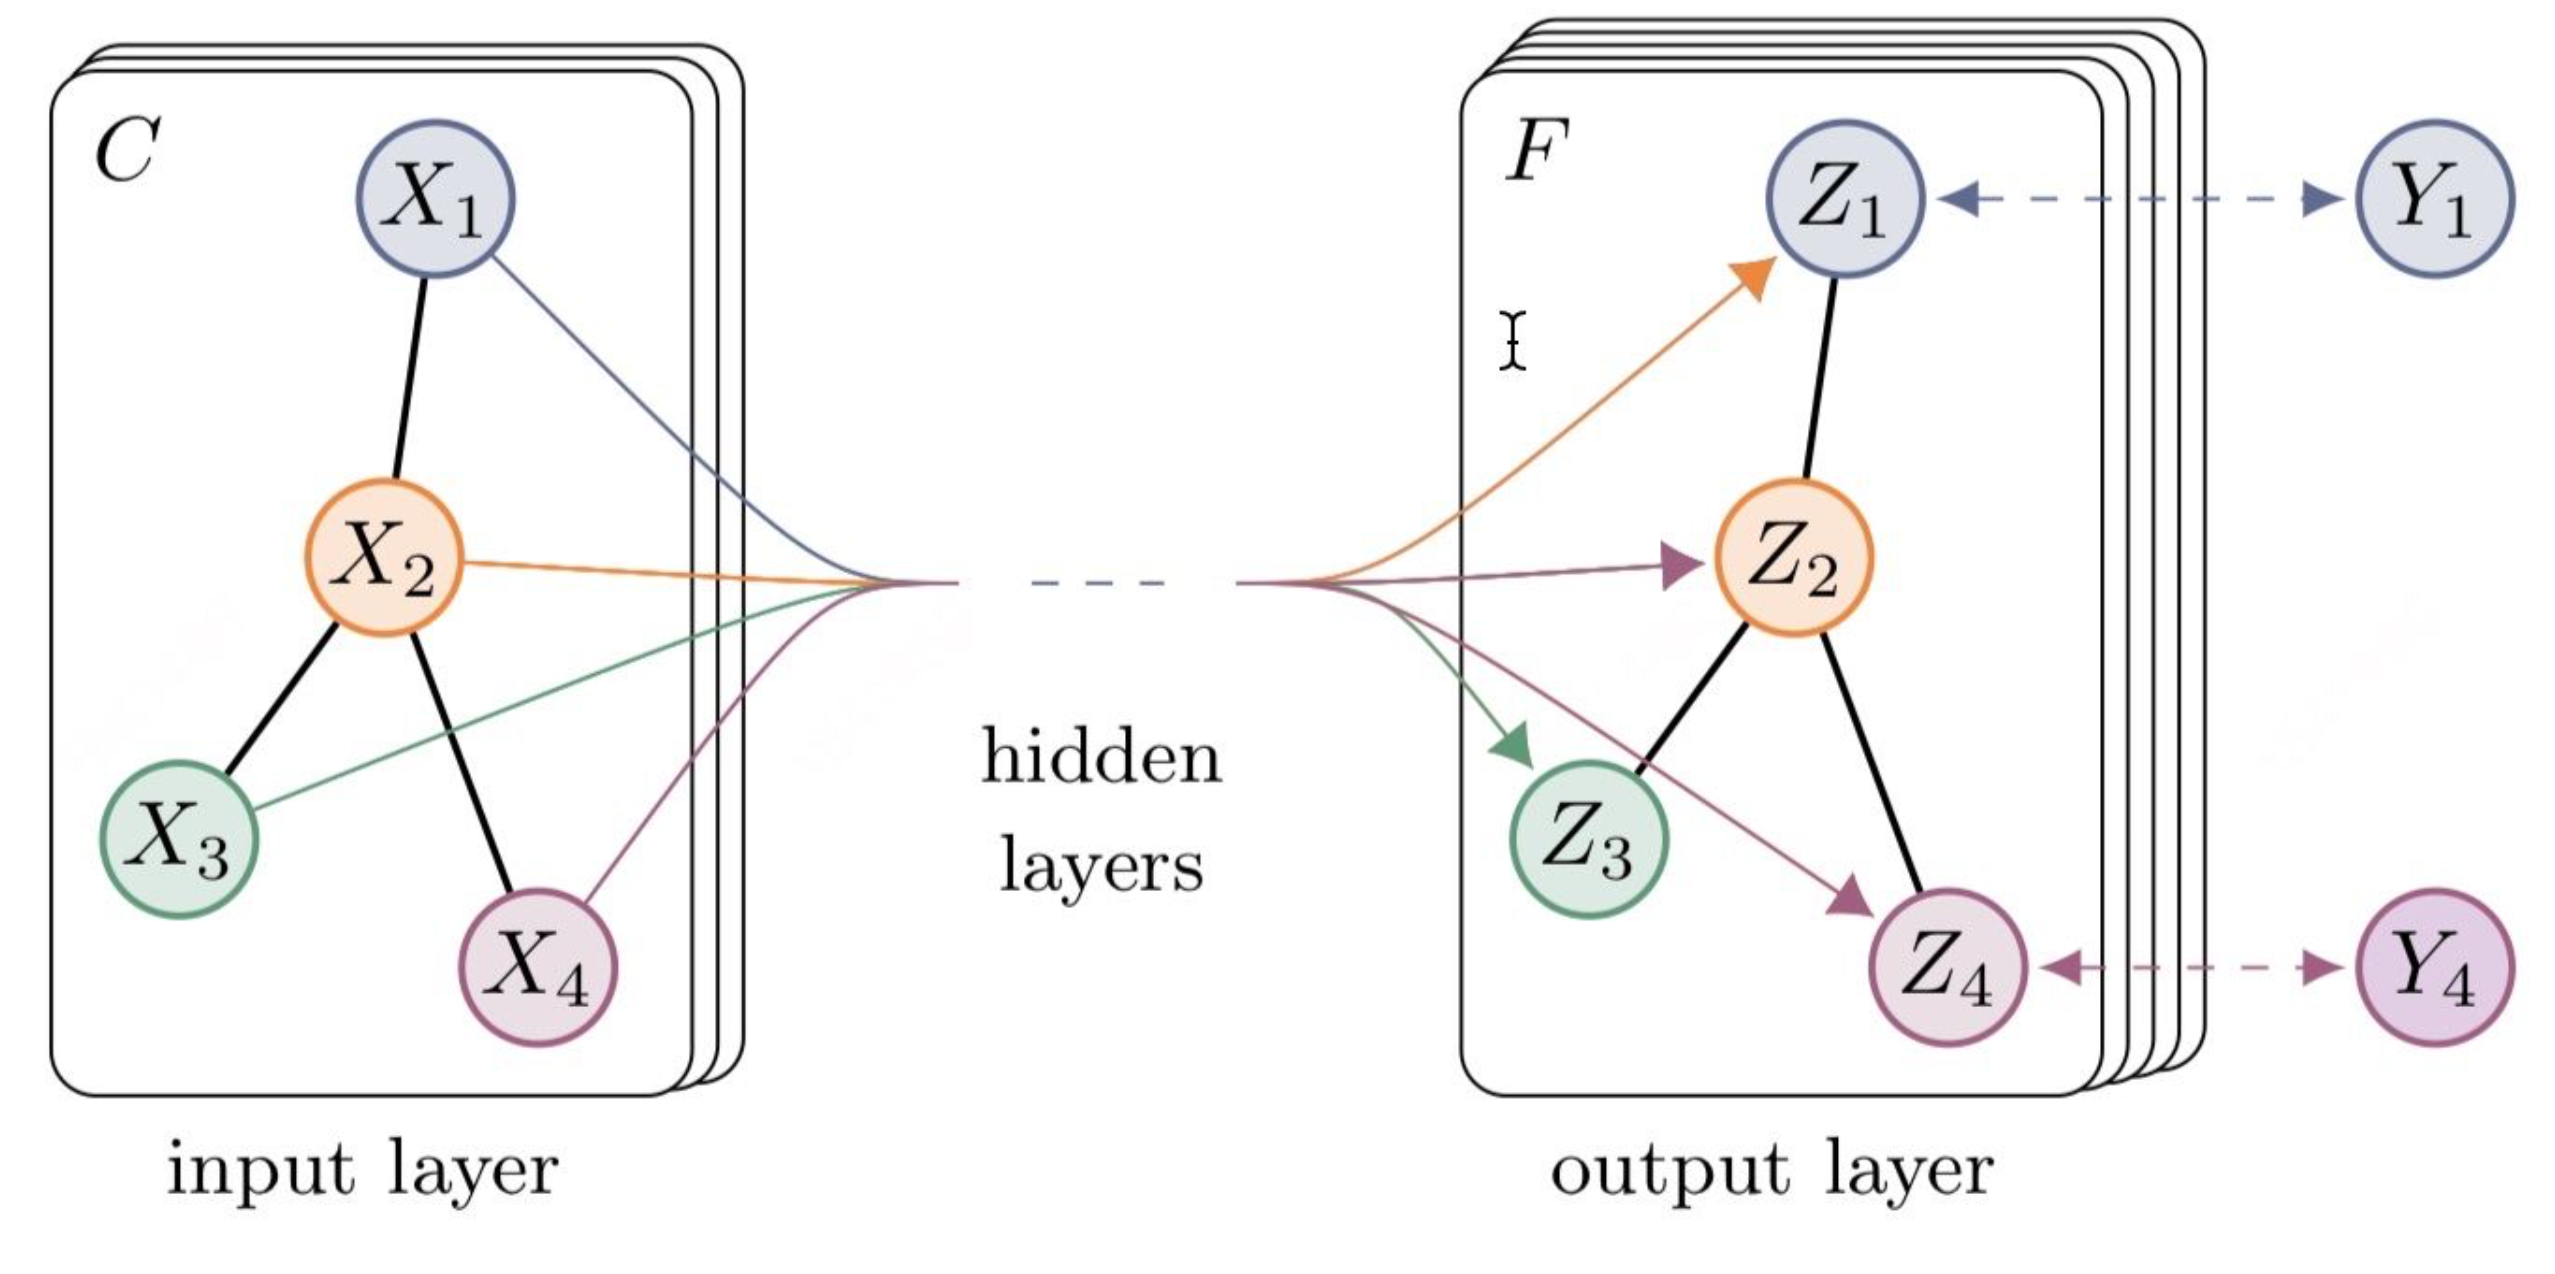
\includegraphics[width=0.80\textwidth]{FigMa/GCN-SEMI.png}\\
    \vspace{-0.3cm}
    \caption{图卷积示意图,来自\parencite{kipf2016semi}}
    \label{fig:GCN-SEMI}
\end{figure}
图\ref{fig:GCN-SEMI}展示了一个标准的GCN。可以看到一个具有个$C$个输入通道的图结构数据通过中间的隐藏层,产生了$D$个通道的输出。在这一过程中,GCN不改变图的空间结构,只是对节点特征进行变换,参考图中各节点的信息流动趋势,捕捉空间结构信息。本文将网络的输入$X$定义为一个$V*D$的矩阵,其中$V$代表输入图中的节点数量,而$D$代表输入图中节点的特征维度。$X$经过特征处理后即可得到输出$Z$,一个维度为$V*D^{\prime}$的矩阵,其中$V$结构不变,$D^{\prime}$为变换后的特征维度。

一个图的空间结构可以用邻接矩阵描述。邻接矩阵是一种用于表示图形或网络的数据结构。它是一个方阵,其中行和列分别对应于图中的节点,矩阵中的每个元素表示两个节点之间是否存在一条边。具体来说,假设图有$V$个节点,那么邻接矩阵的大小为$V \times V$。如果节点$i$和节点$j$之间存在一条边,则邻接矩阵中第$i$行第$j$列的元素为1;如果它们之间不存在边,则该元素为0。邻接矩阵还可以用于表示带权图,其中矩阵中的元素表示边的权重。如果节点$i$和节点$j$之间存在一条权重为$w$的边,则邻接矩阵中第i行第j列的元素为$w$;如果它们之间不存在边,则该元素为0或一个特殊的表示不存在边的值(如-1)。邻接矩阵是一种简单且直观的图表示方法,适用于图比较稠密(边数接近节点数的平方)的情况。但是,对于稀疏图(边数远小于节点数的平方)来说,邻接矩阵会浪费大量的空间。此时,邻接矩阵的时间和空间复杂度可能较高,因此在应用时需要针对稀疏矩阵进行额外的优化。在定义邻接矩阵以后,可以很轻易重构一个图结构。本文用$G=(V,E)$定义一个图,其中$V$代表节点,$E$代表边。通过$\left|V\right| \times \left|V\right|$得到$A$,其中如果节点$i$和节点$j$之间存在联系,则$A_{ij}=1$否则则等于0。由此,便通过一个图数据结构得到邻接矩阵$A$,同理也可以根据$A$得到一个图数据结构。
\begin{figure}[ht]
    \centering
    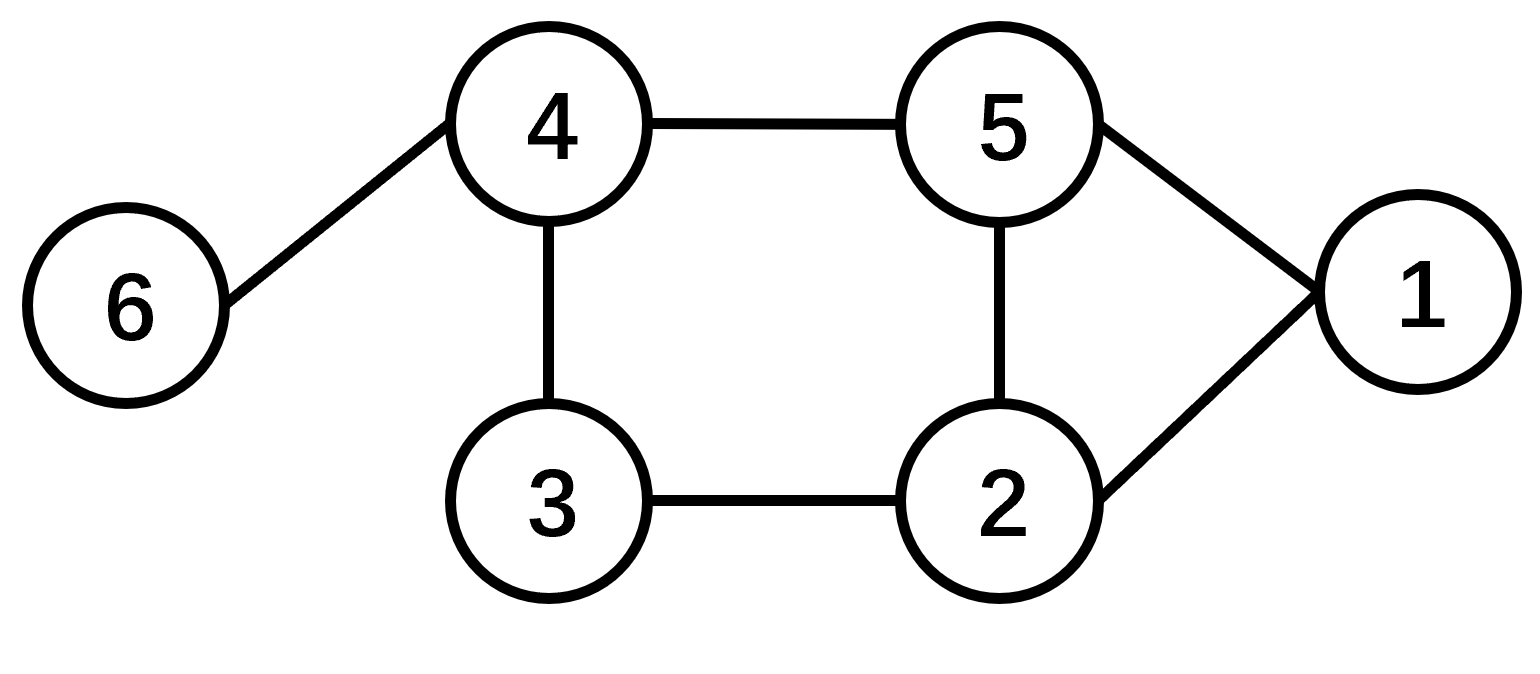
\includegraphics[width=0.70\textwidth]{FigMa/Graph_structure.png}\\
    \vspace{-0.3cm}
    \caption{图结构数据示意图}
    \label{fig:Graph_structure}
\end{figure}
如上图所示,本文定义了一个拥有6个节点的图结构数据。其中节点上的数字代表该节点的编号,节点间的连接代表两点间存在联系。根据上文,可以将该图的数据结构以邻接矩阵的形式表示如下。
\begin{equation}
\begin{pmatrix}
        0 & 1 & 0 & 0 & 1 & 0 \\
        1 & 0 & 1 & 0 & 1 & 0 \\
        0 & 1 & 0 & 1 & 0 & 0 \\
        0 & 0 & 1 & 0 & 1 & 1 \\
        1 & 1 & 0 & 1 & 0 & 0 \\
        0 & 0 & 0 & 1 & 0 & 0 \\
\end{pmatrix}
\label{equation:adj_mat}
\end{equation}
其中有联系的关节点则被置为1。例如,由于1号节点和5号节点之间存在连接,则$A_{15}$和$A_{51}$均被置为1且因为图\ref{fig:Graph_structure}为无向无环图,因此邻接矩阵沿着对角线对称,对角线上的元素均为0。所以可以根据邻接矩阵将图卷积网络中的一层定义为如下非线性函数:
\begin{equation}
   H^{(l+1)} = f(H^{(l)} ,A)
    \label{equation:GCN_simple_define}
\end{equation}
其中$H$为该层的隐变量,其中输入层$H(0)=X$,输出层$H(L)=Z$,L代表最后一层,$Z$为最终输出网络的结果。不同的GCN函数,使用不同的GCN模型$f(\cdot,\cdot)$。被广泛传播的图卷积层定义如下:
\begin{equation}
    f(H^{(l)},A) = \sigma\left( \hat{D}^{-\frac{1}{2}} \hat{A} \hat{D}^{-\frac{1}{2}} H^{(l)}W^{(l)} \right)
    \label{equation:GCN_define}
 \end{equation}
其中$D$代表图结构的度矩阵,$W$为每一个卷积层的权重,该公式的物理含义为,当前层隐变量是由上一层隐变量以邻接矩阵为权重加权求和后,再经过线性变换$W$和激活函数得到的。

为了方便理解,本文先定义一个简单的函数$f(H^{(l)},A)$为基础,逐渐推导得到公式\ref{equation:GCN_define}。本文首先定义一个简单的图卷积层级传导公式:
\begin{equation}
    f(H^{(l)},A) = \sigma\left( {A}H^{(l)}W^{(l)} \right)
    \label{equation:GCN_define_base}
 \end{equation}
 在公式\ref{equation:GCN_define_base}中本文通过$A$和$H$矩阵相乘的形式完成简单的加权求和计算。然后再由权重矩阵$W$对节点特征维度进行变换,最后通过激活层$\sigma$得到该层的特征矩阵。$AH$的直观理解是,将与自身相邻的节点特征(信息)加权求和后得到更新后的特征。

 但在这一过程中,更新后的特征只包含周围节点的信息,不包括自身的原始信息(因为邻接矩阵中对角线元素为0,即图中不存在自身回环。)。为此,可以另$\hat{A} = A + I$向邻接矩阵中手动添加自身回环。其中$I$为单位矩阵。此外,如果要进行加权求和,则必须保证权值和为1,否则特征数值会迅速膨胀。因此还需要对$\hat{A}$进行归一化。本文对$\hat{A}$中每一行除以该行的和,即该节点的度。于是$\hat{A}$被归一化为$\hat{D}^{-1}\hat{A}$,在实际操作中通常使用对称归一化,于是便得到了公式\ref{equation:GCN_define}中的邻接矩阵$\hat{D}^{-\frac{1}{2}}\hat{A}\hat{D}^{-\frac{1}{2}}$。代入公式\ref{equation:GCN_define_base}即可得到图卷积公式\ref{equation:GCN_define}。在理解图卷积的直观意义和公式由来后。接下来,本文将借助拉普拉斯算子给出公式\ref{equation:GCN_define}的推导过程以及数学含义,从数学的角度解释图卷积网络的设计逻辑。
\section{拉普拉斯算子}
为了推导图卷积网络,本文将首先介绍拉普拉算子(Laplace operator)作为铺垫,进而给出图卷积网络的数学定义。拉普拉斯算子被定义为欧几里得空间中,一个二阶可微函数$f$梯度的散度,即对该函数求二阶微分,结果表示为$\Delta f$其中$\Delta$代表拉普拉斯算子。如果$f$是图上定义的一组高维向量,则$Lf$是在图空间求二阶微分,其中$L$为拉普拉斯矩阵。为了叙述方便,本文首先在连续欧式空间中,定义$f(x,y,z)$为一个二阶可微的三元函数,在该函数上分别对梯度和散度进行定义。

\subsection{连续空间中的拉普拉斯算子}
梯度是一个矢量,表示某一函数在沿着该点的方向导数上可以取得局部极值。即函数在该方向上沿着该方向下降速度最快,变化率最大。对于位于欧式空间中,一阶可微的函数$f(x,y,z)$。在该函数上一点$P(x,y,z)$,称向量:
\begin{equation}
    \left\{ \frac{\partial f}{\partial x}, \frac{\partial f}{\partial y}, \frac{\partial f}{\partial z} \right\}= \frac{\partial f}{\partial x}\vec{i} + \frac{\partial f}{\partial y}\vec{j} + \frac{\partial f}{\partial z}\vec{k}
    \label{equation:grad}
\end{equation}
为$f(x,y,z)$在点$P$处的梯度,记为$gradf(x,y,z)$或$\nabla f(x,y,z)$,其中$\nabla = \frac{\partial}{\partial x}\vec{i} + \frac{\partial}{\partial y}\vec{j} + \frac{\partial}{\partial z}\vec{k}$。

散度($\nabla \cdot$ )被定义为空间中各矢量场的发散程度,某点的散度被定义为$div(F)$,散度大于零的点代表该点向周围散播能量,而散度小于零的点代表该点向周围吸收能量。当某点散度为0时,则代表该点既不发散也不吸收能量,为无源点。

在了解散度和梯度在连续函数空间中的定义后,即可给出连续二阶可微函数空间中,拉普拉斯算子的具体定义。对于三维函数$f(x,y,z)$,拉普拉斯算子被定义为梯度($\nabla f$)的散度($\nabla \cdot$)。$\Delta f = \nabla^2 f = \nabla \cdot \nabla f = div(grad f)$,在笛卡尔坐标系下被表示为公式\ref{equation:laplace_operator}$(a)$,从三维拓展到在$n$维空间后,拉普拉斯算子被表示为公式\ref{equation:laplace_operator}$(b)$:
\begin{equation}
    \begin{aligned}
        \Delta f &= \frac{\partial^2 f}{\partial x^2}, \frac{\partial^2 f}{\partial y^2}, \frac{\partial^2 f}{\partial z^2} (a)
        \\
        \Delta &= \sum_{i=1}^{n} \frac{\partial^2}{\partial x^2_i} (b)
   \end{aligned}
    \label{equation:laplace_operator}
\end{equation}

\subsection{离散空间中的拉普拉斯算子}\label{discrate_laplace}
在公式\ref{equation:laplace_operator},本文给出了在连续二阶可微函数上的拉普拉斯算子定义。然而,图卷积网络所处理的图结构数据位于离散空间中,需要进一步给出离散空间中的拉普拉斯算子。本文首先从一维离散空间中进行推导。对于位于一维离散空间中的函数$f(x)$,设离散函数空间中的最小间隔为$h$,则$f(x)$在$x_i$处的一阶微分为:

\begin{equation}
    f(x_i)^{\prime} = \frac{ f(x_{i+1}) - f(x_{i+1}) }{2h} 
    \label{equation:frist_order}
\end{equation}

使用同样的方法计算$f(x)$在$x_i$处的二阶微分,可得:
\begin{equation}
    f(x_i)^{\prime \prime} = \frac{ f(x_{i+1}) + f(x_{i+1}) - 2f(x_i) }{h^2} 
    \label{equation:second_order}
\end{equation}

在一维基础上进行推广,可以获得拉普拉斯算子在离散二维空间上的表达式,公式\ref{equation:2d_laplace}展示了离散二维空间中的函数$f(x,y)$的拉普拉斯算子表达式。

\begin{equation}
    \begin{aligned}
        \Delta f &= \frac{\partial^2 f}{\partial x^2} + \frac{\partial^2 f}{\partial y^2} \\
        &= f(x+1, y) + f(x-1, y) - 2f(x, y) + \\
        &\ f(x, y+1) + f(x, y-1) + 2f(x, y) \\
        &= f(x+1, y) + f(x-1, y) + \\
        &\ f(x, y+1) + f(x, y-1) - 4f(x,y)
    \end{aligned}
    \label{equation:2d_laplace}
\end{equation}

由公式\ref{equation:2d_laplace}可以直观地看到,对于离散二维空间中的点$(i,j)$, 该点的拉普拉斯算子值由该点和四个方向上的相邻点的特征值之差得到。这代表拉普拉斯算子可以描述相邻离散点之间的信息差异,反映了信息的流动趋势。当$\Delta f > 0$表示该点的信息将会流向相邻节点,当$\Delta f < 0$时,四周节点的信息流向该节点,当$\Delta f = 0$时,则关节点间不发生信息流动。由于拉普拉斯算子可以很好的描述离散节点间的信息流动方向和强度。因此,在图卷积网络中被用来描述相邻关节点间的信息流动趋势,具体方式本文将在下一章详细叙述如何使用拉普拉斯算子推导图卷积网络公式。当前,本文首先给出图结构数据下的拉普拉斯算子定义。

对具有$V$个节点的图$G$,本文将其定义为一个$V$维的向量$G=(x_1, \cdots, x_V, E)$,$x_i$表示第$i$个节点的特征值,$E$为边的集合,通过公式\ref{equation:2d_laplace}将图结构数据中的拉普拉斯算子定义为:
\begin{equation}
    \begin{aligned}
        \Delta x_i &= \sum_{j \in V}A_{ij}(x_i - x_j) \\
        &=\sum_{j \in V}A_{ij}x_i - \sum_{j \in V}A_{ij}x_j \\
        &= d_i x_i - A_{i:}H
    \end{aligned}
    \label{equation:nd_laplace}
\end{equation}
其中$d_i$是节点$x_i$的度。$A_{i:} = (A_{i1},\cdots, A_{iV})$, $H = (x_1, \cdots, x_V)^T$,$A_{i:}H$为这两个向量的内积。

公式\ref{equation:nd_laplace}仅仅给出了单个节点拉普拉斯算子的计算方法,本文将其推广到图中的所有节点,以矩阵形式表示拉普拉斯算子,该矩阵则被称为拉普拉斯矩阵。
\begin{equation}
    \begin{aligned}
        \Delta G &= \left(  \begin{array}{cccc}
            \Delta x_1 \\
            \vdots \\
            \Delta x_V
         \end{array} \right) = 
         \left(  \begin{array}{cccc}
            d_1x_1 - A_{1:}H \\
            \vdots \\
            d_Vx_V - A_{V:}H
         \end{array} \right)
        \\
        & =diag(d_i)H - AH \\
        & = (D-A)H \\
        & = L(G)
    \end{aligned}
    \label{equation:nd_laplace_mat}
\end{equation}

公式\ref{equation:nd_laplace_mat}给出了图结构数据中的拉普拉斯矩阵$L(G)$。其中$D$为度矩阵,$A$为邻接矩阵,它将作为图卷积网络中的重要组成部分。

\section{图卷积网络推导}
在\ref{discrate_laplace}节中,本文得到了图结构数据$G$的拉普拉斯矩阵$L(G) = (D-A)H$,对该拉普拉斯矩阵进行对称归一化后可得:
\begin{equation}
    \begin{aligned}
        L^{norm} &= D^{-\frac{1}{2}}L D^{-\frac{1}{2}} \\
        &= D^{-\frac{1}{2}}(D-A)D^{-\frac{1}{2}} \\
        &= I - D^{-\frac{1}{2}}A D^{-\frac{1}{2}}
    \end{aligned}
    \label{equation:norm_laplace}
\end{equation}
该归一化矩阵,对角线为1,非对角线为$-\frac{1}{\sqrt{deg(x_i)deg(x_j)} }$。

本文希望通过傅里叶级数处理图卷积过程,可两个函数的卷积定义如下:
\begin{equation}
    f*g = \mathcal{F}^{-1}\{\mathcal{F}\{f\} \cdot \mathcal{F} \{ g \} \}
    \label{equation:f_convolution}
\end{equation}
其中$\mathcal{F}$为傅里叶级数。假设$L(G)$的特征值为$\Lambda$,特征向量为$U$。在图卷积网络中,傅里叶变换对应$\mathcal{G}\mathcal{F}\{x\} = U^Tx$,对应的其逆变换为$\mathcal{I}\mathcal{G}\mathcal{F}\{x\} = Ux$,将二者代入公式\ref{equation:f_convolution}中即可得到对应的图卷积公式。
\begin{equation}
    \begin{aligned}
        g * x &= \mathcal{I}\mathcal{G}\mathcal{F}\{ \mathcal{G}\mathcal{F}\{g\} \cdot \mathcal{G}\mathcal{F}\{x\} \} \\
        &=U(U^Tg \cdot U^Tx) 
    \end{aligned}
    \label{equation:gcn_f}
\end{equation}
本文将$g$定义为一个以拉普拉斯矩阵为参数的函数$g(L)$,其作用是传播或接受周围邻居的信息。因为有$U^T L = U^T U \Lambda U^T = \Lambda U^T$,所以本文进一步将$U^T g$看作是以拉普拉斯矩阵特征值为参数的函数$g_\theta(\Lambda) = diag(\theta)$,其中$\theta$为参数。随后,在频率域上,公式\ref{equation:gcn_f}可以简化表示为:
\begin{equation}
    g_\theta x= Ug_\theta U^T x
    \label{equation:gcn_f_2}
\end{equation}

为了简化计算,本文采用$Chebyshev \ polynomials$将$g_\theta$近似为:
\begin{equation}
    g_{\theta^{\prime}} * x \approx \sum_{k=0}^{K} \theta^{\prime}_k T_k (\widetilde{\Lambda})  
    \label{equation:g_approx}
\end{equation}

其中$\widetilde{\Lambda} = \Lambda - I$,$K$表示经过了$K$阶拉普拉斯矩阵的处理。$T_k(x) = 2xT_{k-1}(x) - T_{k-2}(x)$,同时$T_0 = 1$,$T_1 = x$。上述近似计算代入公式\ref{equation:gcn_f_2}可得:

\begin{equation}
    \begin{aligned}
        g_\theta x &= Ug_\theta U^T x \\
        &\approx U \sum_{k=0}^{K} \theta^{\prime}_k T_k (\widetilde{\Lambda}) U^Tx
        &=\sum_{k=0}^{K} \theta^{\prime}_k T_k (U\widetilde{\Lambda}U^T)x
        &=\sum_{K}^{k=0} \theta^{\prime}_k T_k(\widetilde{L})x
    \end{aligned}
    \label{equation:gcn_3}
\end{equation}
其中$\widetilde{L} = L - I$,由于一个GCN只包含一次信息传递过程,只拥有一个一阶的拉普拉斯矩阵,因此取$k=1$代入公式\ref{equation:gcn_3},可得到如下所示的图卷积计算公式:
\begin{equation}
    \begin{aligned}
        g_\theta x &=\sum_{1}^{k=0} \theta^{\prime}_k T_k(\widetilde{L})x \\
        &=\theta^{\prime}_0 T_0(L-I)x + \theta^{\prime}_1 T_1(L-I)x \\ 
        &=\theta^{\prime}_0x + \theta^{\prime}_1(L-I)x\\
        &=\theta^{\prime}_0x + \theta^{\prime}_1(I-D^{-\frac{1}{2}}AD^{-\frac{1}{2}}-I)x\\
        &=\theta^{\prime}_0x - \theta^{\prime}_1 D^{-\frac{1}{2}}AD^{-\frac{1}{2}} x
    \end{aligned}
    \label{equation:gcn_4}
\end{equation}

为了减少参数和降低模型复杂度,设$\theta = \theta^{\prime}_0 = -\theta^{\prime}_1$,同时令$\hat{A} = I+A$和$\hat{D}_ii = \sum_{j \in V}\hat{A}_ij$,可得:
\begin{equation}
        g_\theta * x =\theta \hat{D}^{-\frac{1}{2}}\hat{A} \hat{D}^{-\frac{1}{2}} x
    \label{equation:gcn_5}
\end{equation}

再加上激活函数$\sigma$,即可得到\ref{gcn_model_define}节中提到的图卷积模型计算公式:
\begin{equation}
    f(H^{(l)},A) = \sigma\left( \hat{D}^{-\frac{1}{2}} \hat{A} \hat{D}^{-\frac{1}{2}} H^{(l)}W^{(l)} \right)
    \label{equation:GCN_define_2}
 \end{equation}

其中$H$为输入的特征向量,$W$代表参数$\theta$。在实际使用中,为了降低模型的复杂度,通常将$A$定义为可学习的参数矩阵,由网络进行归一化,因此模型被简化为:

\begin{equation}
    f(H^{(l)},A) = \sigma\left(\hat{A}H^{(l)}W^{(l)} \right)
\end{equation}


\subsection{总结}
在本章节中,本文介绍了图卷积的基本概念,包括图结构、拉普拉斯算子、谱理论和特征表示等。拉普拉斯算子是图卷积的核心概念之一,通过计算它可以得到图的特征表示。接着,本文又推导了图卷积公式,介绍了如何使用卷积神经网络在图上进行卷积操作,进一步拓展了图卷积的应用。

首先,图卷积是一种用于处理图数据的卷积操作,可以用于学习图的结构信息。其次,拉普拉斯算子是计算图卷积的核心算子之一,它可以将图的结构信息转化为数学表达形式,为图卷积提供了理论基础。第三,谱理论是图卷积的重要理论基础之一,通过它可以了解拉普拉斯算子的性质和作用。最后,特征表示是图卷积的重要应用之一,它可以将图的信息转化为向量表示,方便进行机器学习任务的处理。

在对基本的图卷积网络知识进行一定的一定的铺垫后,在后续的内容中,本文将详细介绍提出的基于渐进式策略的人体运动姿态预测算法,主要包含训练策略和网络结构设计两部分
。
% 参考文章
% https://zhuanlan.zhihu.com/p/85287578
% https://zhuanlan.zhihu.com/p/107162772